When the user wants to augment their dataset, Karma needs to first search for available object and class properties.  
To do so, the user first selects a node in their source model to search against, in this case E21\_Person1 in Figure~\ref{fig:simple-model-screenshot}.
Karma creates a list of classes to search against that contains the class assigned to the node by either the user or Karma and any other parent classes Karma can reason about from the user provided ontologies.  
Karma then searches the model repository for other source models that describe entities of the same classes.  This is accomplished by issuing SPARQL queries against R2RML mappings that capture the source models.  

Specifically, Karma looks for TriplesMaps with SubjectMaps that have rr:class properties values in common with the search class list.  
Once Karma finds a set of candidate TriplesMaps, it parses the TriplesMaps' PredicateObjectMaps to extract object and data properties.  
The predicate is taken from the PredicateObjectMap's rr:predicate value.  
If the PredicateObjectMap contains a simple ObjectMap, then Karma has discovered a data property.  
If it contains a RefObjectMap, then Karma has found an object property and then returns the object's class by following the rr:parentTriplesMap link to a TriplesMap and then a SubjectMap.  
Karma presents these to the users as outgoing links to augment their node with.  
It is also necessary to find properties where the node the user has selected is the object, or incoming links.  
To do so, Karma follows a similar path, but returns the rr:class and rr:predicate from a TriplesMap with a PredicateObjectMap that has a rr:parentTriplesMap that links to TriplesMaps that describe the search classes. 
Once Karma has identified the possible properties according to the models in the properties, the user can chose from the presented properties and then have Karma augment their dataset as illustrated in Figure~\ref{fig:search-screenshot}.

\begin{figure*}
\begin{center}
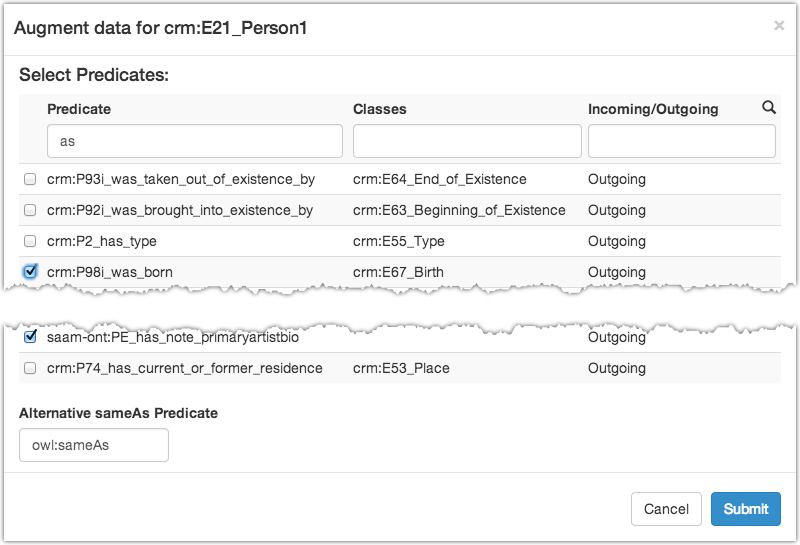
\includegraphics[width=4.9in]{images/5-search.png}
\vspace{-3mm}
\caption{CIDOC CRM object and data properties discovered from other sources for the user to augment E21\_Person}
\vspace{-2mm}
\label{fig:search-screenshot}
\end{center}
\vspace{-1.5em}
\end{figure*}


